\documentclass[tikz,border=8pt]{standalone}
% Shared look for every TikZ diagram. Load with \input{../../tools/tikz-style.tex}
\usepackage[T1]{fontenc}
\usepackage{lmodern}
\renewcommand{\sfdefault}{lmr}  % diagrams use the same serif as the text
\usetikzlibrary{arrows.meta, positioning, shapes.geometric, calc, fit, backgrounds}
\definecolor{cblue}{HTML}{4C78A8}
\definecolor{corange}{HTML}{F58518}
\definecolor{cgreen}{HTML}{54A24B}
\definecolor{cred}{HTML}{E45756}
\definecolor{cpurple}{HTML}{B279A2}
\definecolor{cgrey}{HTML}{6B6B6B}
\tikzset{
  every picture/.style={font=\sffamily, line width=1.2pt},
  box/.style={draw=#1, fill=#1!12, rounded corners=4pt, align=center, inner sep=7pt, minimum height=1.1cm},
  box/.default=cgrey,
  arrow/.style={-{Stealth[length=3mm]}, draw=cgrey, line width=1.4pt},
  title/.style={font=\sffamily\bfseries\Large},
  note/.style={font=\sffamily\small, text=cgrey, align=center},
}
\AtBeginDocument{\hyphenpenalty=10000 \exhyphenpenalty=10000}

\begin{document}
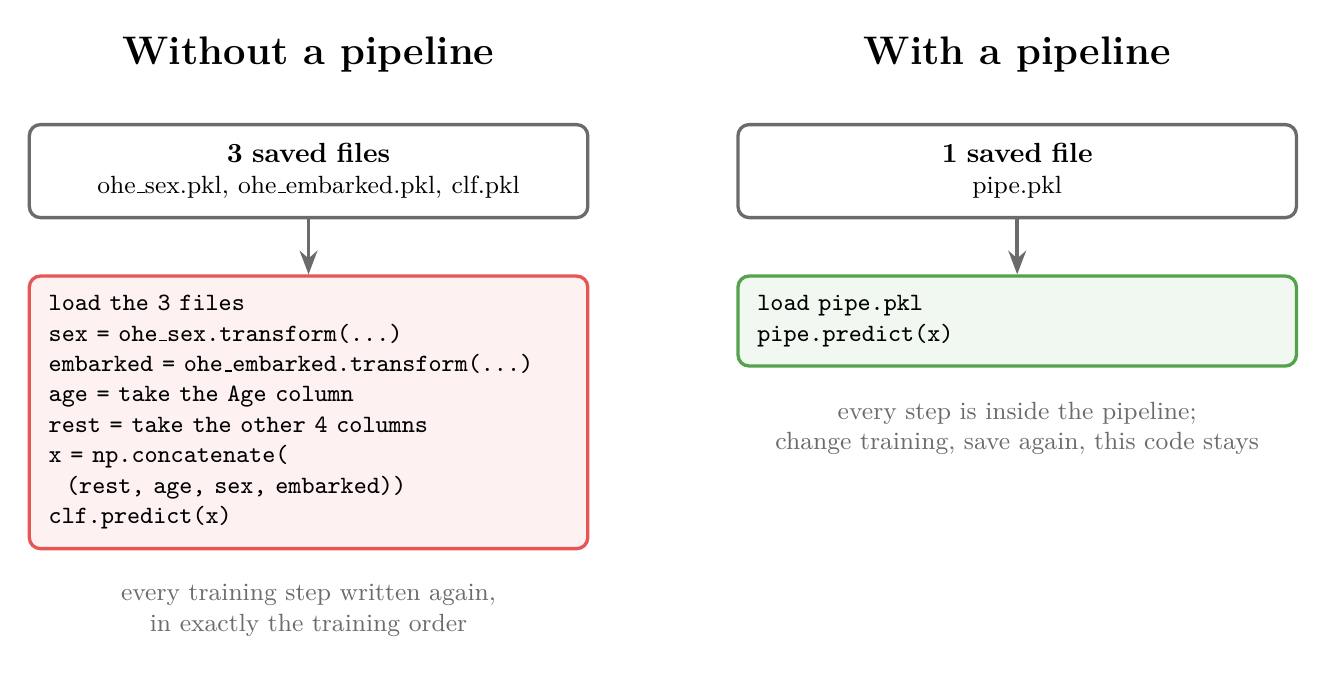
\begin{tikzpicture}[code/.style={draw=#1, fill=#1!8, rounded corners=4pt, align=left, inner sep=7pt, font=\ttfamily\small, text width=6.6cm}]
  % left: without a pipeline
  \node[title] (h1) at (0,0) {Without a pipeline};
  \node[box=cgrey, fill=white, text width=6.6cm, below=0.5cm of h1] (f1) {\textbf{3 saved files}\\[-1pt]\small ohe\_sex.pkl, ohe\_embarked.pkl, clf.pkl};
  \node[code=cred, below=0.7cm of f1] (c1) {%
    load the 3 files\\
    sex = ohe\_sex.transform(...)\\
    embarked = ohe\_embarked.transform(...)\\
    age = take the Age column\\
    rest = take the other 4 columns\\
    x = np.concatenate(\\
    \ \ (rest, age, sex, embarked))\\
    clf.predict(x)};
  \draw[arrow] (f1) -- (c1);
  \node[note, text width=6.6cm, below=0.3cm of c1] {every training step written again,\\in exactly the training order};
  % right: with a pipeline
  \node[title] (h2) at (9,0) {With a pipeline};
  \node[box=cgrey, fill=white, text width=6.6cm, below=0.5cm of h2] (f2) {\textbf{1 saved file}\\[-1pt]\small pipe.pkl};
  \node[code=cgreen, below=0.7cm of f2] (c2) {%
    load pipe.pkl\\
    pipe.predict(x)};
  \draw[arrow] (f2) -- (c2);
  \node[note, text width=6.6cm, below=0.3cm of c2] {every step is inside the pipeline;\\change training, save again, this code stays};
\end{tikzpicture}
\end{document}
